% Options for packages loaded elsewhere
\PassOptionsToPackage{unicode}{hyperref}
\PassOptionsToPackage{hyphens}{url}
%
\documentclass[
  12pt,
]{article}
\usepackage{amsmath,amssymb}
\usepackage{lmodern}
\usepackage{iftex}
\ifPDFTeX
  \usepackage[T1]{fontenc}
  \usepackage[utf8]{inputenc}
  \usepackage{textcomp} % provide euro and other symbols
\else % if luatex or xetex
  \usepackage{unicode-math}
  \defaultfontfeatures{Scale=MatchLowercase}
  \defaultfontfeatures[\rmfamily]{Ligatures=TeX,Scale=1}
\fi
% Use upquote if available, for straight quotes in verbatim environments
\IfFileExists{upquote.sty}{\usepackage{upquote}}{}
\IfFileExists{microtype.sty}{% use microtype if available
  \usepackage[]{microtype}
  \UseMicrotypeSet[protrusion]{basicmath} % disable protrusion for tt fonts
}{}
\makeatletter
\@ifundefined{KOMAClassName}{% if non-KOMA class
  \IfFileExists{parskip.sty}{%
    \usepackage{parskip}
  }{% else
    \setlength{\parindent}{0pt}
    \setlength{\parskip}{6pt plus 2pt minus 1pt}}
}{% if KOMA class
  \KOMAoptions{parskip=half}}
\makeatother
\usepackage{xcolor}
\IfFileExists{xurl.sty}{\usepackage{xurl}}{} % add URL line breaks if available
\IfFileExists{bookmark.sty}{\usepackage{bookmark}}{\usepackage{hyperref}}
\hypersetup{
  pdftitle={Combining medium-intensity tillage to improve soil compaction and infiltration with cover crop mixes to suppress weeds},
  pdfkeywords={urban, compact, weed, till, cover, water},
  hidelinks,
  pdfcreator={LaTeX via pandoc}}
\urlstyle{same} % disable monospaced font for URLs
\usepackage[margin=1in]{geometry}
\usepackage{longtable,booktabs,array}
\usepackage{calc} % for calculating minipage widths
% Correct order of tables after \paragraph or \subparagraph
\usepackage{etoolbox}
\makeatletter
\patchcmd\longtable{\par}{\if@noskipsec\mbox{}\fi\par}{}{}
\makeatother
% Allow footnotes in longtable head/foot
\IfFileExists{footnotehyper.sty}{\usepackage{footnotehyper}}{\usepackage{footnote}}
\makesavenoteenv{longtable}
\usepackage{graphicx}
\makeatletter
\def\maxwidth{\ifdim\Gin@nat@width>\linewidth\linewidth\else\Gin@nat@width\fi}
\def\maxheight{\ifdim\Gin@nat@height>\textheight\textheight\else\Gin@nat@height\fi}
\makeatother
% Scale images if necessary, so that they will not overflow the page
% margins by default, and it is still possible to overwrite the defaults
% using explicit options in \includegraphics[width, height, ...]{}
\setkeys{Gin}{width=\maxwidth,height=\maxheight,keepaspectratio}
% Set default figure placement to htbp
\makeatletter
\def\fps@figure{htbp}
\makeatother
\setlength{\emergencystretch}{3em} % prevent overfull lines
\providecommand{\tightlist}{%
  \setlength{\itemsep}{0pt}\setlength{\parskip}{0pt}}
\setcounter{secnumdepth}{5}
\newlength{\cslhangindent}
\setlength{\cslhangindent}{1.5em}
\newlength{\csllabelwidth}
\setlength{\csllabelwidth}{3em}
\newlength{\cslentryspacingunit} % times entry-spacing
\setlength{\cslentryspacingunit}{\parskip}
\newenvironment{CSLReferences}[2] % #1 hanging-ident, #2 entry spacing
 {% don't indent paragraphs
  \setlength{\parindent}{0pt}
  % turn on hanging indent if param 1 is 1
  \ifodd #1
  \let\oldpar\par
  \def\par{\hangindent=\cslhangindent\oldpar}
  \fi
  % set entry spacing
  \setlength{\parskip}{#2\cslentryspacingunit}
 }%
 {}
\usepackage{calc}
\newcommand{\CSLBlock}[1]{#1\hfill\break}
\newcommand{\CSLLeftMargin}[1]{\parbox[t]{\csllabelwidth}{#1}}
\newcommand{\CSLRightInline}[1]{\parbox[t]{\linewidth - \csllabelwidth}{#1}\break}
\newcommand{\CSLIndent}[1]{\hspace{\cslhangindent}#1}
\usepackage{booktabs}
\usepackage{longtable}
\usepackage{array}
\usepackage{multirow}
\usepackage{wrapfig}
\usepackage{float}
\usepackage{colortbl}
\usepackage{pdflscape}
\usepackage{tabu}
\usepackage{threeparttable}
\usepackage{threeparttablex}
\usepackage[normalem]{ulem}
\usepackage{makecell}
\usepackage{xcolor}
\ifLuaTeX
  \usepackage{selnolig}  % disable illegal ligatures
\fi

\title{Combining medium-intensity tillage to improve soil compaction and infiltration with cover crop mixes to suppress weeds}
\author{true \and true \and true}
\date{}

\begin{document}
\maketitle
\begin{abstract}
Urban soils have been degraded by decades of industrial activities, but they also represent opportunities to improve food sovereignty for urban residents practicing urban agriculture.
Urban growers often use varying practices of compost, tillage, and cover cropping, but without distinguishing their benefits to optimize integrated approaches.
This study examined how tillage methods representing various intensities and cover crop mixes targeting different functions affected agricultural variables including soil compaction, water infiltration rate, herbaceous weedy plant pressure, and crop yield.
Results showed that both roto- and tractor-till significantly affected compaction but not yield compared to no-till, and roto-till also improved infiltration, while tractor-till reached deeper soils but allowed denser weed growth.
Mixing sorghum-sudangrass, buckwheat, and cowpea cover crops significantly reduced weed pressure compared to other mixtures, and perennials affected compaction but not soil water infiltration under no-till.
These results reveal that medium-intensity tillage may offer more balanced trade-offs for initial management, and that cover crops can help reduce weeds under low-till strategies.
Overall this study offers evidence detailing effects of various tillage and cover crop styles that can be of use for smallholder urban growers.
\end{abstract}

{
\setcounter{tocdepth}{2}
\tableofcontents
}
\hypertarget{introduction}{%
\section{Introduction}\label{introduction}}

Urban soils have the potential to improve the livelihoods of most of the world \emph{(\protect\hyperlink{ref-acuto18}{Acuto, Parnell, and Seto 2018})} via implications for climate adaptation, erosion and storm-water runoff management, and local forestry \emph{(\protect\hyperlink{ref-pavao-zuckerman08}{Pavao-Zuckerman 2008})}, but many urban soils are in poor health for cultivation after decades of industrial use, including sealing and structural engineering \emph{(\protect\hyperlink{ref-lal15}{Lal, Negassa, and Lorenz 2015})}.
This is especially notable in post-industrial cities of the mid-western USA, where many vacant lots remain on soils can have relatively high compaction, pH, and chemical contamination \emph{(\protect\hyperlink{ref-beniston16}{Beniston, Lal, and Mercer 2016})}.
Degraded urban soils with low organic matter are also likely far from organic carbon saturation \emph{(\protect\hyperlink{ref-stewart07}{C. E. Stewart et al. 2007})}, making the potential benefit from tailored agricultural management large \emph{(\protect\hyperlink{ref-kumar16}{Kumar and Hundal 2016}; \protect\hyperlink{ref-kuzyakov19}{Kuzyakov and Zamanian 2019})}.
However, popular single strategies like organic compost amendments to urban gardens, while widely beneficial across many physical, chemical, and biological properties \emph{(\protect\hyperlink{ref-cogger05}{Cogger 2005})}, can also have other side effects like excess phosphorus \emph{(\protect\hyperlink{ref-small19}{Small et al. 2019})}, which highlights the benefits of new and ongoing research studies of urban soil management, especially of integrated approaches for soil multi-functionality \emph{(\protect\hyperlink{ref-blesh17}{Blesh 2017})} including cover cropping, tillage, diverse mulching, and others.
In response to various needs, urban agriculture continues to expand as local communities and non-profit organizations revitalize and establish a diversity of new green initiatives including landscaping to improve local access to healthy food and a cleaner and safer environment \emph{(\protect\hyperlink{ref-block12}{Block et al. 2012}; \protect\hyperlink{ref-clendenning16}{Clendenning, Dressler, and Richards 2016}; \protect\hyperlink{ref-garcia-sempere19}{García-Sempere et al. 2019}; \protect\hyperlink{ref-siebert20}{Siebert 2020})}.
Urban growers in particular often invest relatively large amounts of money, time, and resources from accessible capital into amending soils for vegetable production \emph{(pers. comms.)},
thereby improving the potential impact of research for promising accessible urban soil remediation strategies, which remains limited beyond compost \emph{(\protect\hyperlink{ref-grossman03}{Grossman 2003})}.

Mechanized tilling has long been a regular strategy improve short-term arability, among others like adding compost, although research studies increasingly report soil degradation after long-term and intensive tillage.
Short-term tillage benefits include larger soil pores and lower soil bulk density \emph{(\protect\hyperlink{ref-hill85}{Hill, Horton, and Cruse 1985}; \protect\hyperlink{ref-badalikova10}{Badalíková 2010})}, and potentially more available nutrients \emph{(\protect\hyperlink{ref-wolkowski90}{Wolkowski 1990})} with less potential weed regeneration \emph{(\protect\hyperlink{ref-barberi01}{Barberi and Lo Cascio 2001}; \protect\hyperlink{ref-cordeau20}{Cordeau, Baudron, and Adeux 2020})}, making tillage useful against soil compaction and associated water infiltration and drainage issues, which can facilitate faster seeding and crop establishment early in the season \emph{(\protect\hyperlink{ref-monti01}{Monti, Venturi, and Elbersen 2001})}.
However, longer-term side effects of excessive and/or very intensive tillage include weaker soil aggregate stability and structure \emph{(\protect\hyperlink{ref-six02a}{Six et al. 2002}; \protect\hyperlink{ref-catania18}{Catania et al. 2018})}, increasing dependence on tillage to maintain past yields \emph{(\protect\hyperlink{ref-decarcer19}{de Cárcer et al. 2019})}, and faster soil erosion \emph{(\protect\hyperlink{ref-richter21}{Richter 2021})}, which has more recently led to events like the USA Dust Bowl, and historically poses an existential threat to agricultural societies when combined with other stressors \emph{(\protect\hyperlink{ref-lal07}{Lal 2007}; \protect\hyperlink{ref-montgomery07}{Montgomery 2007}; \protect\hyperlink{ref-amundson15}{Amundson et al. 2015})}.
In response, sustainable and regenerative agriculture theories promote no-till or minimal-till management approaches like broadfork tools to re-focus on soil health and fertility \emph{(\protect\hyperlink{ref-wang06}{Wang et al. 2006}; \protect\hyperlink{ref-roger-estrade10}{Roger-Estrade et al. 2010})}, which comes with different challenges like stronger pressure from weeds \emph{(\protect\hyperlink{ref-anderson07}{Anderson 2007})}, highlighting a role for continuing research into diverse no-till strategies.
For urban growers, machinery can also be cost-prohibitive, and limited access to agricultural loans \emph{(\protect\hyperlink{ref-daniel07}{Daniel 2007})} has resulted in affected communities adapting by organizing equipment sharing systems, which can be more practical in denser urban housing arrangements compared to diffuse rural ones.
This variation in accessibility of machinery can promote mixed tillage strategies by urban growers including tractor- and/or roto-till, which likely have different effects on soil and weed issues, but there remains little public documentation comparing benefits of various tillage styles on remediating urban soils \emph{(\protect\hyperlink{ref-bazzoffi98}{Bazzoffi 1998}; \protect\hyperlink{ref-materechera09}{Materechera 2009})}, which slows the innovation of tailored management strategies for the array of urban grower goals.

Cover cropping has been another long-recommended strategy of sustaining longer-term yields by maintaining soil fertility \emph{(\protect\hyperlink{ref-perez21}{Perez 2021}; \protect\hyperlink{ref-richter21}{Richter 2021})}, although current strategies could be improved from relying on single species to designing complementary species mixes.
The namesake benefit of cover crops is to cover the soil in areas without active cultivation, which maintains root activity and weakens erosion \emph{(\protect\hyperlink{ref-garcia-gonzalez18}{García-González et al. 2018})}, but different species will also vary in the benefits they can provide based on physiological traits.
For example, legumes like cowpea (or black-eyed peas, \emph{Vigna unguiculata subsp. unguiculata}), clovers (\emph{Trifolium sp.}), and hairy vetch (\emph{Vicia villosa}) are popular cover crops because of their additional symbioses with root bacteria that fix nitrogen from the air into soils where it is more available for future crop use \emph{(\protect\hyperlink{ref-grossman05}{Grossman et al. 2005})}.
Similarly, buckwheat helps scavenge soil phosphorus \emph{(\protect\hyperlink{ref-possinger13}{Possinger, Byrne, and Breen 2013})}, which is often a limiting macro-nutrient in clay soils \emph{(\protect\hyperlink{ref-mori22}{Mori et al. 2022})}, and could also be combined with compost that is usually high in phosphorus to address recurring soil phosphorus deficiencies.
Other plants, including grasses like sorghum (\emph{Sorghum bicolor}), tend to grow deep roots, or have other traits like allelopathic chemical defenses, that compete with weeds enough to keep them suppressed over time \emph{(\protect\hyperlink{ref-weston89}{Weston, Harmon, and Mueller 1989})}.
Broader implications of cover cropping also include higher soil organic matter, though the underlying processes remain complex \emph{(\protect\hyperlink{ref-king20}{King 2020})}, and few studies show direct correlations between soil organic matter and yield \emph{(\protect\hyperlink{ref-oldfield19}{Oldfield, Bradford, and Wood 2019})}.
Furthermore, while large rural organic farms can benefit from incorporating specifically-chosen cover cropping into their mechanized operations, the reliance of urban agriculture more on labor over machinery offers an opportunity to develop new cover cropping systems that combine seeding and terminating different species together to improve the potential efficiency of soil remediation efforts.
For example, sorghum, cowpea, and buckwheat could be combined into a mixed strategy that can increase soil nitrogen, soil phosphorus, and suppress weeds via deep and shallow roots with allelopathic chemical defenses, although cover crop synergisms generally remain understudied \emph{(\protect\hyperlink{ref-mead81}{Mead and Riley 1981}; \protect\hyperlink{ref-bedoussac15}{Bedoussac et al. 2015}; \protect\hyperlink{ref-bourke21}{Bourke et al. 2021})}.
An integrated complex approach to optimizing cover cropping systems including interspecific species interactions are well-posed to be validated by research studies in urban agriculture followed by adaptation to rural agriculture, and even international implications \emph{(\protect\hyperlink{ref-stewart13}{R. Stewart et al. 2013})}.

In this study, we investigated how different tillage techniques and cover crop species mixes affect soil physical properties and yield.
Tillage methods ranged from high disturbance using a tractor and implements to minimal disturbance with a broadfork.
Cover crop species mixes were selected based on target functions including reducing compaction, suppressing weeds, and perenniality, or potential for sustainable re-growth.
We hypothesized that both tillage and cover crop mixing would confer similar benefits to soil functions, which would translate to weed pressure and yield.
Accordingly, we predicted that roto-till, a moderate soil disturbance, would best balance compaction and weed pressure benefits, deepening where soil hardpan layers occur that limit root penetration, and thereby increase soil water infiltration rates, and also reduce weed cover, density, and diversity.
We also expected that the cover crop mix designed against soil compaction would have the deepest soil harpan depth and highest water infiltration rates compared to other mixes, mostly due to the deeper rooting potential by forage radish (\emph{Raphanus sativus var. longipinnatus}) and ryegrass (\emph{Secale cereale}).
Finally we expected that the cover crop mix designed for weed suppression would experience the lowest local weed cover, density, and diversity, due to allelopathic chemical defense traits from buckwheat (\emph{Fagoprum esculentum}) and surghum-sudangrass (\emph{Sorghum bicolor x Sorghum bicolor var. sudanese}).

\hypertarget{methods}{%
\section{Methods}\label{methods}}

\hypertarget{site}{%
\subsection{Site}\label{site}}

The study site was located at the Michigan State University (MSU) - Detroit Partnership for Food, Learning, and Innovation (DPFLI) (42.4, -83.3), a 1.6-ha (4 acres) extension facility dedicated to urban agriculture and engaging with local small-scale growers in Detroit, MI, USA.
The climate is temperate with four seasons, with mean annual temperature of \textasciitilde9.5 C (49.1 F) and precipitation at \textasciitilde787 mm (31 in) (\url{ncdc.noaa.gov}).
The site was formerly a school building and associated playground until 2016 when it was demolished \textbf{after closing for \ldots{} reasons} and the land became vacant.
The habitat is \textasciitilde1.2 km (\textasciitilde0.8 mi) away from a small river, conferring some wetland ecosystem properties like denser soils.
It is also surrounded by sealed sidewalk and small roads on all four sides, which likely affects runoff and drainage patterns (Fig \ref{fig:plots}a).
\includegraphics{merge_files/figure-latex/plots-1.pdf}

Site soils can be classified as Technosols (Fig \ref{fig:plots}b), given that large metal artifacts can be found throughout various profiles \emph{(\protect\hyperlink{ref-fao14}{FAO 2014})}, from when the area was filled in with nearby soils during highway road construction, as was common in mid-western USA industrial manufacturing cities many decades ago in the \emph{1960s} \emph{(\protect\hyperlink{ref-beniston16}{Beniston, Lal, and Mercer 2016})}.
Accordingly, the growing area has both a finer- and coarser-textured side (Fig \ref{fig:plots}a),
and this study was done on the side with consistent clay of \textasciitilde37\%.
Topsoil A horizons are 1-2'' (\textless5 cm) deep, and subsoil B horizons can be \textgreater30.5 cm (1 ft) deep, with a muted yellow color \textbf{YR\#\#?!} (Fig \ref{fig:plots}b).
A baseline site-level soil lab assessment from Cornell determined that the top \emph{4 in (10 cm)} of soils around the site together have relatively good organic matter at
\textasciitilde2.5 ±
0.3\%
and nutrient levels, including concentrations of heavy metals like lead and arsenic \textbf{(Table ??)} which were present below harmful government human-contact standards (\url{cfpub.epa.gov/ecotox}).
The soils were also assesed to have decent but sub-optimal \emph{CO\textsubscript{2}} respiration rates of
0.2 ±
0 mg per day
(Table \ref{tab:chem}.
Some main concerns limiting productivity include high alkaline pH of
8.1 ±
0.1,
lowering availability of existing nutrients, as well as weak aggregate stability of
19 ±
4.4,
leading to concerns with aeration, infiltration, rooting, crusting when dry, erosion, and runoff (Table \ref{tab:chem}).

\begin{table}

\caption{\label{tab:chem}Baseline Cornell Soil Health Assessment}
\centering
\begin{tabular}[t]{c|c|c}
\hline
Variable & Median & Deviation\\
\hline
\multicolumn{3}{l}{\textbf{Biological}}\\
\hline
\hspace{1em}Organic Matter (\%) & 2.5 & 0.3\\
\hline
\hspace{1em}Respiration (mg per day) & 0.2 & 0.0\\
\hline
\multicolumn{3}{l}{\textbf{Physical}}\\
\hline
\hspace{1em}Aggregate Stability (\%) & 19.0 & 4.4\\
\hline
\multicolumn{3}{l}{\textbf{Chemical}}\\
\hline
\hspace{1em}pH & 8.1 & 0.1\\
\hline
\hspace{1em}Phosphorus (ppm) & 2.2 & 1.0\\
\hline
\hspace{1em}Potassium (ppm) & 103.8 & 36.3\\
\hline
\multicolumn{3}{l}{\textbf{-- minor}}\\
\hline
\hspace{1em}\hspace{1em}Iron (ppm) & 6.0 & 4.4\\
\hline
\hspace{1em}\hspace{1em}Magnesium (ppm) & 463.6 & 24.9\\
\hline
\hspace{1em}\hspace{1em}Manganese (ppm) & 42.1 & 4.9\\
\hline
\hspace{1em}\hspace{1em}Zinc (ppm) & 3.8 & 2.9\\
\hline
\end{tabular}
\end{table}

\hypertarget{design}{%
\subsection{Design}\label{design}}

The study area was a 278 \emph{m\textsuperscript{2}} (2992.4 \emph{ft\textsuperscript{2}}) section on the East side of the site that was divided into 36 separate 4.6 \emph{m\textsuperscript{2}} (49.5 \emph{ft\textsuperscript{2}}) plots in nine rows and four columns (Fig \ref{fig:plots}c).
Tillage groups spanned the nine columns in adjacent groups of three, while cover crop mix treatments spanned the rows with one row per cover crop mix, totaling 26 plots, or 12 plots per tillage group and nine plots per cover crop mix.
Before applying treatments, approximately 0.2 \emph{m\textsuperscript{3}} (8.5 \emph{ft\textsuperscript{3}}) of compost was incorporated into each plot.

\textbf{One aggregated sample per tillage group was collected and analyzed for chemistry using modified Morgan-extractable protocols at the MSU soil test lab (\protect\hyperlink{ref-moebius-clune16}{\textbf{moebius-clune16?}}) and analysis was also conducted on the compost.}

Tillage treatments represented methods of increasing intensity available for small scale agriculture, also varying in cost, machinery needed, and sometimes grower preferences \emph{(\protect\hyperlink{ref-drugova22}{Drugova, Curtis, and Ward 2022})}.
Specifially, treatments included no-till with a broadfork \emph{(NT)}, roto-tiller \emph{(RT)}, and tractor-till \emph{(TT)} with implements.
Tractor-till plots were worked with a subsoiler, moldboard plow, and roto-tiller attached to a tractor up to 30.5 cm (1 ft) deep.
Roto-till plots were treated with a rototiller implement up to 20 cm (7.9 in) deep.
Lastly, no-till plots were worked with only a broadfork up to 10 cm (3.9 in) deep.
All tilling was done once early in the season after compost application.

Cover crop mixes were designed primarily based on plants associated with targeted benefits, and as possible, relative simplicity of re-seeding and winter-kill (e.g.~more heat tolerant) \emph{(\protect\hyperlink{ref-clark07}{Clark 2007})}.
Three mixes were designed to target three functions, with each mix containing three different plant species (Table \ref{tab:crops}).
The mix designed to alleviate compaction generally focused on plants with roots that tend to penetrate and loosen soil well, and ultimately included
crimson clover (\emph{Trifolium incarnatum}),
forage radish (\emph{Raphanus sativus}), and
cereal ryegrass (\emph{Secale cereale})
.
The mix targeting weed suppression included heat- and drought-tolerant crops that tend to grow rapidly, allowing them to outcompete other plants--the taxa chosed were
sorghum-sudangrass (\emph{Sorghum bicolor x Sorghum bicolor var. sudanese}),
cowpea (\emph{Vigna unguiculata subsp. unguiculata}), and
buckwheat (\emph{Fagopyrum esculentum}).
Lastly, a mix was dedicated to perennial cover crops, which in contrast to annuals can survive the winter and thus tend to accumulate biomass and establish before spring weeds--this mix included
hairy vetch (\emph{Vicia villosa}),
red clover (\emph{Trifolium pratense}), and
wheat (\emph{Triticum aestivum}).
We also had a null control group consisting of established vegetation within the plot, where no additional seeds were sown.

\begin{verbatim}
## ==  1 queries  ===============
## ✔  Found:  Hairy+Vetch[Common Name]
## ==  Results  =================
## 
## • Total: 1 
## • Found: 1 
## • Not Found: 0
## ==  1 queries  ===============
## ✔  Found:  Red+Clover[Common Name]
## ==  Results  =================
## 
## • Total: 1 
## • Found: 1 
## • Not Found: 0
## ==  1 queries  ===============
## ✔  Found:  Wheat[Common Name]
## ==  Results  =================
## 
## • Total: 1 
## • Found: 1 
## • Not Found: 0
## ==  1 queries  ===============
## ✔  Found:  Black-Eyed+Pea[Common Name]
## ==  Results  =================
## 
## • Total: 1 
## • Found: 1 
## • Not Found: 0
\end{verbatim}

\begin{table}

\caption{\label{tab:crops}Cover crop mixes}
\centering
\begin{tabular}[t]{c|c|>{}c}
\hline
Function & Plants & Binomial\\
\hline
Weed Suppression & Sorghum-Sudangrass & \em{Sorghum bicolor x S. bicolor var. sudanese}\\
\cline{1-3}
 & Cowpea/Black-Eyed Pea & \em{Vigna unguiculata subsp. unguiculata}\\
\cline{2-3}
\multirow{-2}{*}{\centering\arraybackslash } & Buckwheat & \em{Fagopyrum esculentum}\\
\cline{1-3}
Perennial & Hairy Vetch & \em{Vicia villosa}\\
\cline{1-3}
 & Red Clover & \em{Trifolium pratense}\\
\cline{2-3}
\multirow{-2}{*}{\centering\arraybackslash } & Wheat & \em{Triticum aestivum}\\
\cline{1-3}
Compaction & Forage Radish & \em{Raphanus sativus var. longipinnatus}\\
\cline{1-3}
 & Crimson Clover & \em{Trifolium incarnatum}\\
\cline{2-3}
\multirow{-2}{*}{\centering\arraybackslash } & Cereal Ryegrass & \em{Secale cereale}\\
\cline{1-3}
Null & Existing vegetation (no manipulation) & \em{}\\
\hline
\end{tabular}
\end{table}

\hypertarget{sampling}{%
\subsection{Sampling}\label{sampling}}

Soil compaction was measured with a penetrometer \emph{(AgraTronix \#08180)} in four randomly selected spots within each quarter of every plot, as the depth where resistance was 2 MPa (290.1 psi, \emph{lbs in\textsuperscript{-2}}), which is considered hardpan that roots typically cannot penetrate \emph{(\protect\hyperlink{ref-correa19}{Correa et al. 2019})}.
Measurements were recorded to the nearest \emph{2.5 cm (1 inch)} on dry days in July and October 2019.

Soil water infiltration down to 11.1 cm \emph{(8.75 in)} depth was measured using a 16.5 \emph{(9.5 in)} wide aluminum cylinder, and recording the time up to 160 sec for \emph{1 L (32 fl oz)} to pass through, which represented a typical rainfall amount onto \textasciitilde0.10 \emph{m\textsuperscript{2}} (\textasciitilde1 \emph{ft\textsuperscript{2}}) of soil area (\url{waterdata.usgs.gov}).

Weed pressure was measured using percent cover, richness, and density.
Weed cover was estimated as the total proportion of plot area covered by any weeds,
using a scale of 1-10 with one indicating \textbf{only one species / near zero stems} observed to 10 being \textbf{10 species present / almost the entire plot surface covered at some level with at least part of a weed plant (e.g.~stem or leaf)}.
Weed richness was measured as in other studies \emph{(\protect\hyperlink{ref-storkey18}{Storkey and Neve 2018})} as a unique count of morphospecies observed in each plot.
Weed density was measured as the number of individual stems of either of the two most abundant weed species -- pigweed (\emph{Amaranthus viridis}) and velvetleaf (\emph{Abutilon theophrasti}) -- using a discrete scale in increments of 10 with zero indicating neither species present and five indicating 50 or more total individuals stems of either species.

Five forage radish (Brassica \emph{Raphanus sativus var. longipinnatus}) roots were randomly selected from each plot in the compaction treatment and measured for length, individually, and wet weight, as a cluster.
The length of a radish root was measured from the hypocotyl, or root cap, to where the root became \textasciitilde6.3 mm (\textasciitilde1⁄4 in) wide.

\hypertarget{statistics}{%
\subsection{Statistics}\label{statistics}}

Field space limited strict plot replication for combined treatments (\emph{n}=3), and thus inference from advanced nested mixed models \emph{(\protect\hyperlink{ref-silk20}{Silk, Harrison, and Hodgson 2020})}, so analysis focused on specific hypotheses tested using simpler, more conservative non-parametric tests that make few underlying assumptions about data and thus appropriate for data with lower replication.
Kruskal-Wallis tests were run for tillage and cover crop treatments separately, with alpha corrections from 0.05 to 0.01 under multiple comparisons to descriptively parse any treatment interactions, and overall significant treatment effects were followed up by post-hoc Wilcoxon pairwise tests with Holm-corrected p-value adjustments.
All data were centered at plot-level medians, and where applicable pooled across sampling times given no preliminary significant variation along this axis, together with minimal relevance to focal hypotheses in field studies \emph{(\protect\hyperlink{ref-davies15b}{Davies and Gray 2015})}, and was a general solution to uneven sampling across response variables, minimally increasing statistical power (base \emph{n} ≥ 3-6).
For clarity, results figures were designed to reflect statistical models and grouping transparently.
Significant treatment effect sizes were estimated with \emph{eta\textsuperscript{2}} \emph{(\protect\hyperlink{ref-tomczak14}{Tomczak and Tomczak 2014})} and simpler raw median differences at finer pairwise levels.
All calculations and analyzes were done in R version 4.2.0 (2022-04-22) \emph{(\protect\hyperlink{ref-base}{R Core Team 2022})} with useful functions from the packages \emph{tidyverse} 1.3.1 \emph{(\protect\hyperlink{ref-tidyverse}{Wickham et al. 2019})}, \emph{rstatix} 0.7.0 and \emph{ggpubr} 0.4.0 \emph{(\protect\hyperlink{ref-rstatix}{Kassambara 2021})}.
Data and code are stored at \url{nmedina17.github.com/must},
documented using R packages \emph{here} \emph{(\protect\hyperlink{ref-here}{Müller 2020})}, \emph{bookdown} \emph{(\protect\hyperlink{ref-bookdown2022}{Xie 2022a})}, \emph{measurements} \emph{(\protect\hyperlink{ref-measurements}{Birk 2019})}, \emph{taxize} \emph{(\protect\hyperlink{ref-taxize2020}{Chamberlain et al. 2020})}, \emph{knitr} \emph{(\protect\hyperlink{ref-knitr2022}{Xie 2022b})}, and \emph{rmarkdown} \emph{(\protect\hyperlink{ref-rmarkdown2022}{Allaire et al. 2022})}.

\begin{table}

\caption{\label{tab:pkgsTab}Software packages used}
\centering
\begin{tabular}[t]{l|l|l}
\hline
Package & Version & Citation\\
\hline
base & 4.2.0 & @base\\
\hline
bookdown & 0.26 & @bookdown2016; @bookdown2022\\
\hline
grateful & 0.1.11 & @grateful\\
\hline
here & 1.0.1 & @here\\
\hline
knitr & 1.39 & @knitr2014; @knitr2015; @knitr2022\\
\hline
measurements & 1.4.0 & @measurements\\
\hline
RgoogleMaps & 1.4.5.3 & @RgoogleMaps\\
\hline
rmarkdown & 2.14 & @rmarkdown2018; @rmarkdown2020; @rmarkdown2022\\
\hline
rstatix & 0.7.0 & @rstatix\\
\hline
rticles & 0.23 & @rticles\\
\hline
taxize & 0.9.100 & @taxize2013; @taxize2020\\
\hline
tidyverse & 1.3.1 & @tidyverse\\
\hline
\end{tabular}
\end{table}

\hypertarget{results}{%
\section{Results}\label{results}}

\hypertarget{compaction}{%
\subsection{Compaction}\label{compaction}}

Compaction was affected significantly overall by tillage treatments (
\emph{H} = 38.2,
\emph{df} = 2,
\emph{n} = 72,
\emph{p} = \textless0.0001
) by
\textasciitilde52.4 \%
across cover crop treatments (Fig \ref{fig:compactFig}a).
Tractor-till had the largest significant effect on depth to hardpan compared to no-till (
\emph{p\textsubscript{adj}} = \textless0.0001
),
deepening the depth to hardpan by \textbf{\#\#} cm (conv\_, or \textasciitilde{}\emph{30-100}\%) compared to no-till,
down to
\textasciitilde20.6 ±
4.6 cm
(8.1 ±
1.8 in)
across all cover crop mixes.
Roto-till also had a marginally significant effect on depth to hardpan compared to no-till (
\emph{p\textsubscript{adj}} = 0.1
),
deepening the depth to hardpan by \textbf{\#\#} cm (conv\_, or \textasciitilde{}\emph{0-100}\%) compared to no-till, down to
\textasciitilde13.8 ±
1.9 cm
(5.4 ±
0.7 in).
The overall effect from tillage stemmed from significant effects among the perennial (
\emph{p\textsubscript{adj} = \textless0.01}
) and weed suppression (
\emph{p\textsubscript{adj} = \textless0.01}
) mixes (Fig \ref{fig:compactFig}a).
The effect of roto-till was more pronounced in the perennial mix (
\emph{p\textsubscript{adj} = \textless0.01}
), where depth to hardpan was about twice as deep as in no-till plots (Fig \ref{fig:compactFig}a).
There was also a significant difference of \textbf{\#\#\#} (conv\_, or \textasciitilde{}\emph{33}\%) between tractor- and roto-till among all cover crop mixes (Fig \ref{fig:compactFig}a).

\begin{figure}
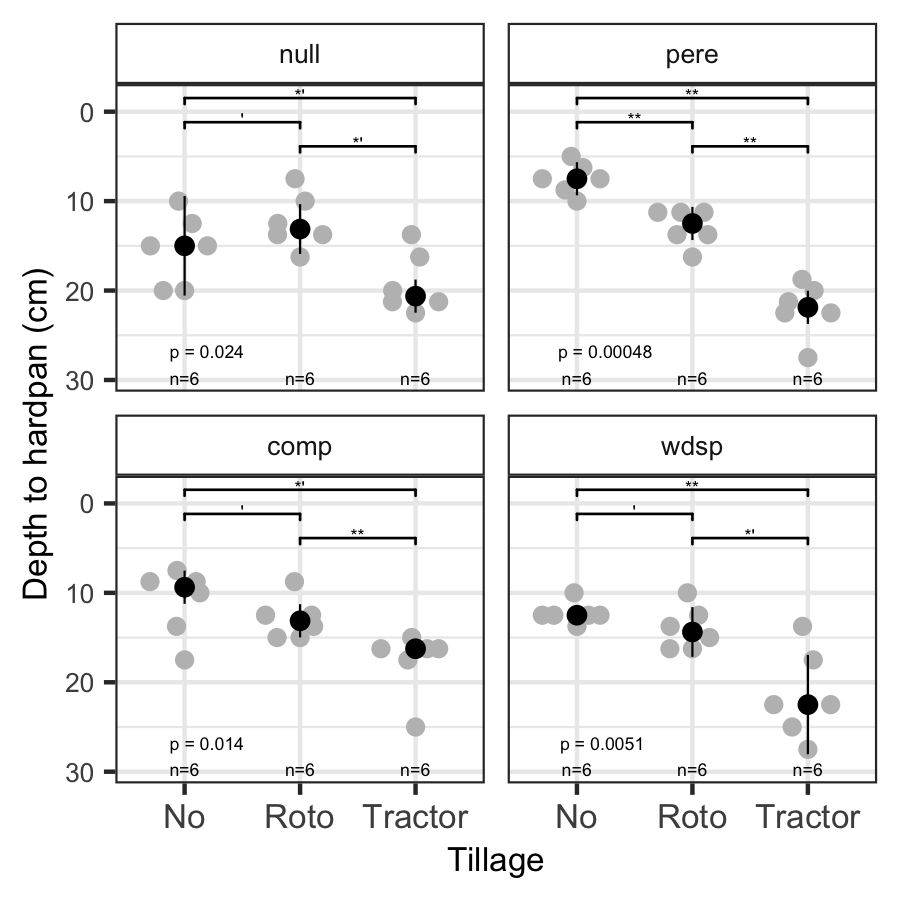
\includegraphics[width=12.5in]{../figs/compactionPlot} \caption{Compaction data (a) , and (b). Significant pairwise post-hoc Wilcoxon test outcomes shown (**** p < 0.0001, *** p < 0.001, ** p < 0.01, * p < 0.05, *' p < 0.1, ' p > 0.1)}\label{fig:compactFig}
\end{figure}

Compaction was not affected by cover crops among tillage groups overall (
\emph{H} = 2,
\emph{df} = 3,
\emph{n} = 72,
\emph{p} = 0.57
), but was significantly affected by cover crops specifically under no-till conditions (
\emph{Holm-corrected alpha = 0.01},
\emph{df = 3},
\emph{n = 6},
\emph{Wilcoxon p\textsubscript{adj} = \textless0.01}
) (Fig \ref{fig:compactFig}b).
Under no-till, the perennial mix had significantly shallower depth to hardpan compared to both null (
\emph{Holm-corrected alpha = 0.01, Wilcoxon p\textsubscript{adj} = \textless0.01}
) and weed suppression mixes (
\emph{Holm-corrected alpha = 0.01, Wilcoxon p\textsubscript{adj} = \textless0.01}
),
raising the depth to hardpan by
\textasciitilde{}\emph{5} cm (
2, or
\textasciitilde{}\emph{30-100}\%
) compared to each mix,
up to
\textasciitilde12.5 ±
7.4 cm
(
4.9 ±
2.9 in
) below the soil surface
(Fig \ref{fig:compactFig}b).

\hypertarget{infiltration}{%
\subsection{Infiltration}\label{infiltration}}

Soil infiltration was significantly affected by tillage (
\emph{H} = 8.5,
\emph{df} = 2,
\emph{n} = 48,
\emph{p} = 0.014
) but not cover crop mix (
\emph{H} = 5.9,
\emph{df} = 3,
\emph{n} = 48,
\emph{p} = 0.12
) (Fig \ref{fig:infilFig}).
Roto-till had significantly faster infiltration compared to no-till (
\emph{p\textsubscript{adj}} = 0
) and marginally significantly compared to tractor-till (
\emph{p\textsubscript{adj}} = 0.1
), speeding up infiltration by
\textasciitilde14.5 \%
compared to each tillage groups,
up to
\textasciitilde{} 13.4 ±
10.7 mL per sec
(
0.2 ±
0.2 in
)
(Fig \ref{fig:infilFig}a).

\begin{figure}
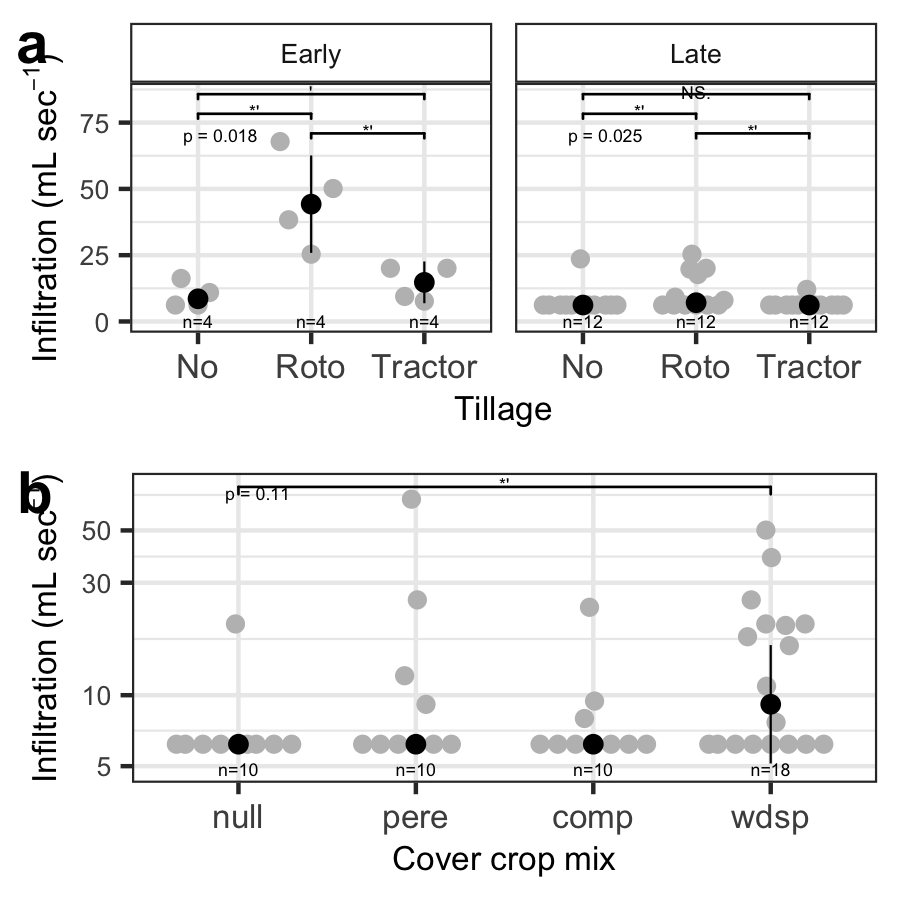
\includegraphics[width=12.5in]{../figs/infilPlot} \caption{Infiltration data (a) , and (b). Significant pairwise post-hoc Wilcoxon test outcomes shown (**** p < 0.0001, *** p < 0.001, ** p < 0.01, * p < 0.05, *' p < 0.1, ' p > 0.1)}\label{fig:infilFig}
\end{figure}

\hypertarget{weed-pressure}{%
\subsection{Weed pressure}\label{weed-pressure}}

Weed density was overall marginally significantly affected by tillage (
\emph{H} = 6.5,
\emph{df} = 2,
\emph{n} = 72,
\emph{p} = 0.039
) by
\textasciitilde25.1 \%,
although weed cover (
\emph{H} = 0.2,
\emph{df} = 2,
\emph{n} = 36,
\emph{p} = 0.92
) and richness (
\emph{H} = 1.6,
\emph{df} = 2,
\emph{n} = 72,
\emph{p} = 0.44
) were not
(Fig \ref{fig:weedsFig}a).
Weeds under tractor-till were marginally significantly denser compared to no-till (
\emph{p\textsubscript{adj}} = 0.1
) and roto-till (
\emph{p\textsubscript{adj}} = 0.1
), denser by
\textasciitilde6.5 \%
compared to each tillage group,
up to
\textasciitilde{} 0.8 ±
0.2 \emph{stems per m\textsuperscript{-2}}
.

\begin{figure}
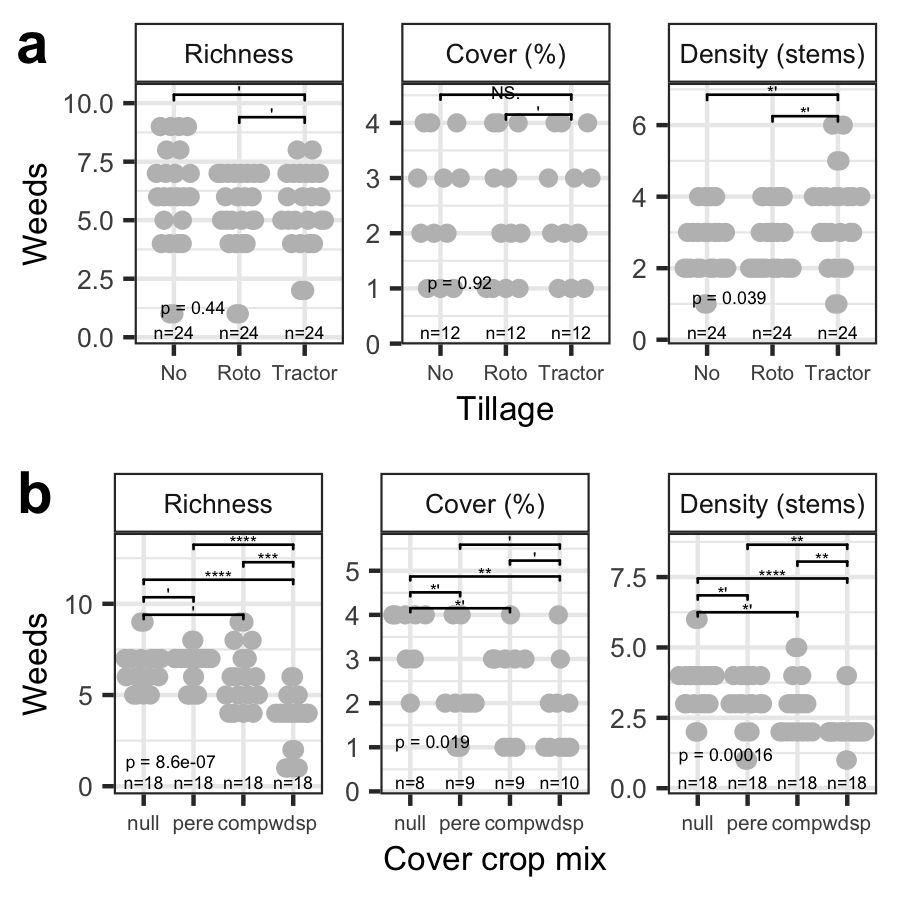
\includegraphics[width=12.5in]{../figs/weedPlot} \caption{Weeds data (a) , and (b). Significant pairwise post-hoc Wilcoxon test outcomes shown (**** p < 0.0001, *** p < 0.001, ** p < 0.01, * p < 0.05, *' p < 0.1, ' p > 0.1)}\label{fig:weedsFig}
\end{figure}

All measured weed variables were affected significantly by cover crop mix, including
weed density (
\emph{H} = 20.1,
\emph{df} = 3,
\emph{n} = 72,
\emph{p} = 0.00016
) changing overall by
\textasciitilde6.5 \%,
weed cover (
\emph{H} = 10,
\emph{df} = 3,
\emph{n} = 36,
\emph{p} = 0.019
) changing overall by
\textasciitilde-5.5 \%, and
weed richness (
\emph{H} = 31,
\emph{df} = 3,
\emph{n} = 72,
\emph{p} = \textless0.0001
) changing overall by
\textasciitilde-0.5 \%
(Fig \ref{fig:weedsFig}b).
Weeds in the null mix covered significantly more plot area compared to the weed suppression mix (
\emph{p\textsubscript{adj}} = 0
) and marginally significantly compared to perennial (
\emph{p\textsubscript{adj}} = 0.1
) and compaction (
\emph{p\textsubscript{adj}} = 0.2
) mixes,
up to
\textasciitilde{} 4 ±
0 \%.
The null mix also had marginally significantly higher weed density compared to the weed suppression mix (
\emph{p\textsubscript{adj}} = 2e-04
) and marginally significantly compared to perennial (
\emph{p\textsubscript{adj}} = 0.2
) and compaction (
\emph{p\textsubscript{adj}} = 0.1
) mixes,
up to
\textasciitilde{} 0.9 ±
0.3 \emph{stems per m\textsuperscript{-2}}.
The weed suppression mix had the most detectable effects on both weed density and richness.
The weed suppression mix significantly lowered weed density compared to all other cover crop mix treatments, namely the null (
\emph{p\textsubscript{adj}} = 2e-04
), perennial (
\emph{p\textsubscript{adj}} = 0
), and compaction (
\emph{p\textsubscript{adj}} = 0.7
) mixes, by
\textasciitilde{} \textbf{\#\#} +-
\textbf{\#\#} (
conv\_, or
\textbf{\%\%\%}
), down to
\textasciitilde{} 0.4 ±
0 \emph{stems per m\textsuperscript{-2}}
.
The weed suppression mix also significantly lowered weed richness compared to all other cover crop mix treatments, namely the null (
\emph{p\textsubscript{adj}} = \textless0.0001
), perennial (
\emph{p\textsubscript{adj}} = \textless0.0001
), and compaction (
\emph{p\textsubscript{adj}} = 0.00093
) mixes, by
\textasciitilde{} \textbf{\#\#} +-
\textbf{\#\#} (
conv\_, or
\textbf{\%\%\%}
), down to
\textasciitilde{} 4 ±
1.5 morphoscpecies taxa
.

\hypertarget{yield}{%
\subsection{Yield}\label{yield}}

Radish yield was not significantly affected by tillage (
\emph{H} = 1.4,
\emph{df} = 2,
\emph{n} = 8,
\emph{p} = 0.5
), and centered at
\textasciitilde{} 13.2 ±
1.5 \emph{kg m\textsuperscript{-2}}
(
29.1 ±
3.3 \emph{lbs m\textsuperscript{-2}}
) and
\textasciitilde{} 0.1 cm
(
0 in
)
long (Fig \ref{fig:yieldFig}).

\begin{figure}
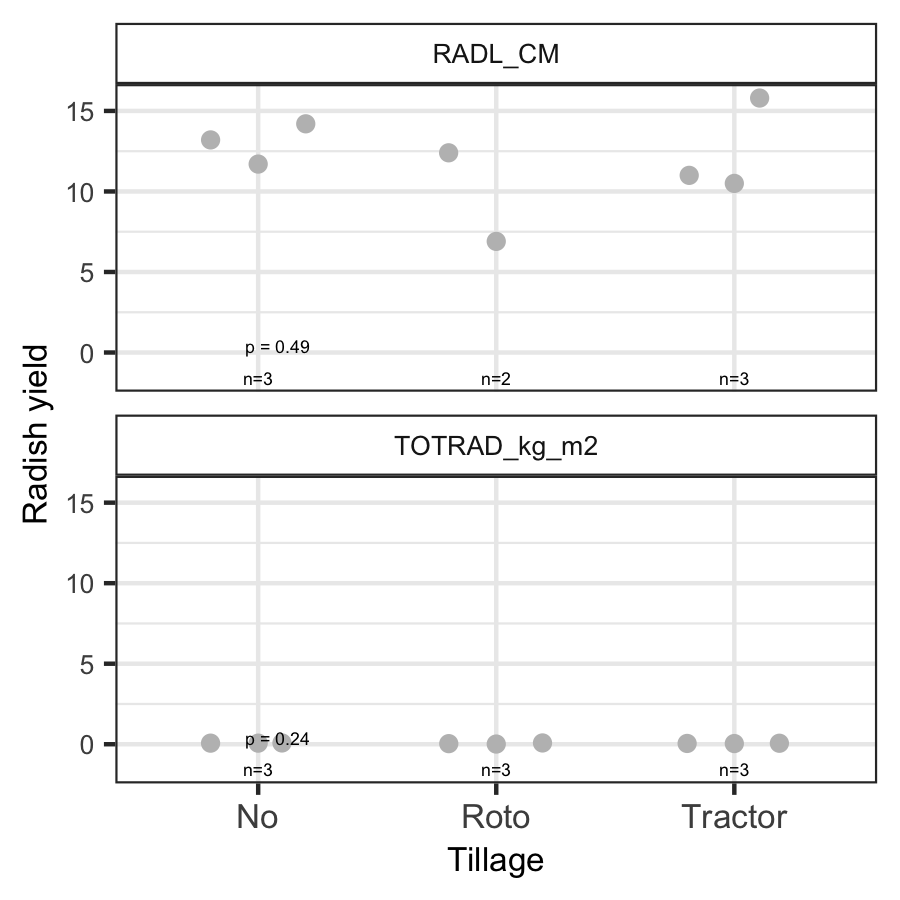
\includegraphics[width=12.5in]{../figs/yieldPlot} \caption{Yield data (a) from no-till and (b) tractor-till. Photo credits: Naim Edwards.}\label{fig:yieldFig}
\end{figure}

\hypertarget{discussion}{%
\section{Discussion}\label{discussion}}

Overall this study informs urban soil management by supporting the use of tillage to address compaction issues and improve infiltration, together with cover crops to also reduce weed pressure.
Our hypothesis was partially supported, because overall tillage significantly deepened the depth to hardpan by \textasciitilde0.5 (Fig \ref{fig:compactFig}a), which was within the range of effect sizes measured among the various cover crop mixes within the no-till treatment (Fig \ref{fig:compactFig}b).
Additionally, infiltration was significantly affected by tillage, with roto-till showing the fastest rates (Fig \ref{fig:infilFig}a), which agreed with our predictions.
Furthermore, weed pressure was significantly affected by both cover crop mixes and tillage (Fig \ref{fig:weedsFig}), although effects from cover crop mixes, especially the weed suppression mix, were more widespread among multiple measured variables (Fig \ref{fig:weedsFig}b).
Despite these significant effects on soils, infiltration, and weeds, yields did not respond to tillage treatments.

Short-term soil compaction issues are commonly alleviated by annual tilling \emph{(\protect\hyperlink{ref-badalikova10}{Badalíková 2010}; \protect\hyperlink{ref-salem15}{Salem et al. 2015})}, and in addition to validating this practice, this study showed that cover cropping can also be used to manage compaction under no-till, although effects vary by mixture of taxa used.
Under tillage, this study validates that tillage intensity corresponds negatively with compaction (measured as depth to hardpan), and additionally clarifies that tractor-till can alleviate compaction in slightly deeper soils below main root zones under
\textasciitilde20.6 ±
4.6 cm
(8.1 ±
1.8 in),
as well as that roto-till can be useful under perennial crops, although under annuals, no-till can be just as effective as roto-till, saving grower time, energy, and cost for areas with crops harvested before rooting surpasses \emph{\textasciitilde10 cm (4 in)} \emph{(\protect\hyperlink{ref-krause95}{Krause and Black 1995})}.
However for urban technosol soils, tilling can beneficially remove large metal artifacts and legacy construction debris like rebar, wires, cables, bricks, cinder blacks, and pipes, all of which could limit root growth under strict no-till management.
Tillage might also obscure cover crop effects on compaction, although cover crops may still provide other benefits, like soil macro-nutrients \emph{(\protect\hyperlink{ref-chapagain20}{Chapagain, Lee, and Raizada 2020})}.
Under no-till, this study found that perennial crop mixes can have significant effects on compaction, but rather than deep roots loosening soils, in some cases depth to hardpan can instead become shallower.
This may be due to dense root mats that can form under grasses \emph{(\protect\hyperlink{ref-douglas92}{Douglas, Koppi, and Moran 1992})} like sorghum-sudangrass, which could further fill already limited pore space in densely-structured clay soils, helping water to pool under the soil surface \emph{(\protect\hyperlink{ref-hoogmoed80}{Hoogmoed and Bouma 1980})}.
Overall other studies have found similar results \emph{(\protect\hyperlink{ref-ozpinar06}{Ozpinar and Cay 2006})}, suggesting short-term benefits of tillage to soil functions (yet long-term costs).

Water infiltration is a key function to improve urban soil functioning for agriculture by minimizing erosion and improving root available water, as well as mitigating storm-water runoff and potentially contaminated flooding \emph{(\protect\hyperlink{ref-masoner19}{Masoner et al. 2019})} that often occurs after short heavy rains, due to soil sealing by concrete near hillslopes \emph{(\protect\hyperlink{ref-dreelin06}{Dreelin, Fowler, and Ronald Carroll 2006})}.
This study found that roto-till resulted in significantly faster infiltration compared to no-till, unlike tractor-till, suggesting that roto-till management can generally be effective for improving infiltration and drainage.
This result could be explained by medium intensity roto-till increasing soil macro-porosity, which compared to soil micro-pores bind water less tightly allowing to flow faster \emph{(\protect\hyperlink{ref-gerke06}{Gerke 2006})}.
In contrast, the tractor diffused tillage energy across deeper soil volume, lowering the density of any added soil macro-pores and thereby making it easier for soil particles to settle back together, whereas no-till may have needed more time to improve macro-porosity via organic matter effects on soil structure \emph{(\protect\hyperlink{ref-king20}{King 2020})}.
It is also possible that this result could be explained by compost incorporation, where tractor-till similarly incorporated compost more diffusely throughout the soil profile, diluting any compost benefits to infiltration.
Against a one inch rain event, this study supported the use of roto-till, but not no-till or tractor-till, which showed rates of only
\textasciitilde{} 6.2 ±
0 mL per sec
(
0.1 ±
0 gal per min
),
which would likely result in runoff pooling in roads and soil erosion.
Regarding cover crops, this study suggests that perennials may not have notable significant effects on infiltration rates, despite detectable effects on compaction.
Based on these findings, roto-till together with compost may be an effective strategy to improve urban soil water infiltration in the short-term, even if no-till may appear to have more evidence as a longer-term strategy \emph{(\protect\hyperlink{ref-cusser20}{Cusser et al. 2020})}.

Weed suppression is important for reducing competition with crops as well as asthma and respiratory health risks from pollen \emph{(\protect\hyperlink{ref-katz14}{Katz and Carey 2014})}, and can also be achieved by tilling \emph{(\protect\hyperlink{ref-barberi01}{Barberi and Lo Cascio 2001}; \protect\hyperlink{ref-cordeau20}{Cordeau, Baudron, and Adeux 2020})}, but this study additionally suggests that cover crops may be more likely to be effective.
Tractor-till, while able to combat relatively deep soil compaction, resulted in the highest weed density of the two most common weeds, velvet leaf (\emph{Abutilon theophrasti}) and pigweed (\emph{Palmer amaranth}), whose root density may have also slowed soil water infiltration rates.
This may have been due to fast-growing weed life histories taking advantage of looser soil, such as to re-sprout clonally, and/or looser soil facilitating the establishment of weed seed banks \emph{(\protect\hyperlink{ref-hesse07}{Hesse, Rees, and Müller-Schärer 2007})}.
However more notably, the targeted weed suppression mix of sorghum-sudangrass, buckwheat, and cowpea significantly reduced both weed density and richness by about half compared to the other cover crop mixes.
This result agrees with other studies pairing buckwheat and sorghum-sudangrass \emph{(\protect\hyperlink{ref-smith15}{Smith, Marín-Spiotta, and Balser 2015})}, and may have occurred due to competitive exclusion by sorghum-sudangrass and/or buckwheat via allelopathic chemical root defenses \emph{(\protect\hyperlink{ref-weston89}{Weston, Harmon, and Mueller 1989})} or competition for light \emph{(\protect\hyperlink{ref-liu09b}{Liu et al. 2009})}, better phosphorus mining and use by buckwheat \emph{(\protect\hyperlink{ref-zhu02}{Zhu et al. 2002})}, facilitation or amplification of these previous effects by cowpea's added nitrogen supply \emph{(\protect\hyperlink{ref-sanginga00}{Sanginga, Lyasse, and Singh 2000}; \protect\hyperlink{ref-martins03}{Martins et al. 2003})}, and/or existing adaptations to poor dry soils \emph{(\protect\hyperlink{ref-barberi18}{Bàrberi et al. 2018})} allowing high biomass accumulation.
Given both effectiveness and relative ease of re-seeding and winter-kill, this weed suppression mix can be used to frame crop beds, keeping out encroaching weeds, or to reduce weed pressure in an area that might be planted in the fall or following season.

Despite overall significant effects by tillage on compaction, infiltration, and weeds, tillage did not significantly affect radish yield.
As is, this study does not rule out more complex relationships between soil compaction, infiltration, and crop yield, as suggested by emerging ideas \emph{(\protect\hyperlink{ref-ryan07}{Ryan, Ludwig, and Mcalpine 2007}; \protect\hyperlink{ref-vandermeer17}{Vandermeer and Perfecto 2017})}.
However, with further replication, it is possible that no-till would show slightly higher yields, validating some similar studies \emph{(\protect\hyperlink{ref-nunes18}{Nunes et al. 2018})}.
Overall yields can respond more to longer-term reservoirs of water and nutrients like mulched compost compared to shorter-term, transient influxes brought by infiltration processes \emph{(\protect\hyperlink{ref-schlegel95}{A. J. Schlegel and Havlin 1995}; \protect\hyperlink{ref-schlegel15}{Alan J. Schlegel et al. 2015})}.
As a result, it is possible that similar alternative soil management practices like no-till combined with compost and mulching application may lead to better yields, although the translation of no-till benefits to soil structure \emph{(\protect\hyperlink{ref-du15}{Du et al. 2015}; \protect\hyperlink{ref-sheehy15}{Sheehy et al. 2015})} on yield are not guaranteed \emph{(\protect\hyperlink{ref-martinez16}{Martínez et al. 2016})} nor do they appear to be widespread \emph{(\protect\hyperlink{ref-pittelkow15}{Pittelkow et al. 2015}; \protect\hyperlink{ref-vandenbygaart16}{VandenBygaart 2016})}.
Additionally, other studies suggest that forage radish can be an effective cover crop in reducing compaction and building soil structure, with minimal or no mechanical tillage \emph{(\protect\hyperlink{ref-chen10b}{Chen and Weil 2010}; \protect\hyperlink{ref-lawley11}{Lawley, Weil, and Teasdale 2011})}.
However ultimately this study suggests the need for future studies of processes tying yield to land management strategies particularly in similar urban clay soils with legacy compaction and pH concerns under smallholder management and possibly including occassional tillage \emph{(\protect\hyperlink{ref-ekboir01}{Ekboir 2001}; \protect\hyperlink{ref-blanco-canqui20}{Blanco-Canqui and Wortmann 2020})}.

Taken together, this study presents data that, in addition to validating previous studies supporting general tillage for short-term soil fertility, also supports the partial use of medium-intensity roto-till and cover crop mixtures \emph{(\protect\hyperlink{ref-chapagain20}{Chapagain, Lee, and Raizada 2020})} specifically for weed suppression.
This study serves as a model demonstration of both widely accessible and effective strategies for growing on re-purposed urban soils after urban land-use turnover.
We advocate for the maximal use of cover crop mixes for various target functions, with medium-intensity tillage to jump-start urban cultivation.

\hypertarget{acknowledgements}{%
\section{Acknowledgements}\label{acknowledgements}}

Thanks to previous anonymous reviewers, and peer student (Kristel, Zach,) discussion of initial drafts.

\hypertarget{funding}{%
\section{Funding}\label{funding}}

\emph{This research did not receive any specific grant from funding agencies in the public, commercial, or not-for-profit sectors.}

\hypertarget{conflicts-of-interest}{%
\section{Conflicts of interest}\label{conflicts-of-interest}}

Authors declare no conflicts of interest.

\hypertarget{data-statement}{%
\section{Data statement}\label{data-statement}}

Data and code available at \url{nmedina17.github.com/must}.

\newpage

\hypertarget{references}{%
\section*{References}\label{references}}
\addcontentsline{toc}{section}{References}

\hypertarget{refs}{}
\begin{CSLReferences}{1}{0}
\leavevmode\vadjust pre{\hypertarget{ref-acuto18}{}}%
Acuto, Michele, Susan Parnell, and Karen C. Seto. 2018. {``Building a Global Urban Science.''} \emph{Nature Sustainability} 1 (1): 2--4. \url{https://doi.org/10.1038/s41893-017-0013-9}.

\leavevmode\vadjust pre{\hypertarget{ref-rmarkdown2022}{}}%
Allaire, JJ, Yihui Xie, Jonathan McPherson, Javier Luraschi, Kevin Ushey, Aron Atkins, Hadley Wickham, Joe Cheng, Winston Chang, and Richard Iannone. 2022. \emph{Rmarkdown: Dynamic Documents for r}. \url{https://github.com/rstudio/rmarkdown}.

\leavevmode\vadjust pre{\hypertarget{ref-amundson15}{}}%
Amundson, Ronald, Asmeret Asefaw Berhe, Jan W. Hopmans, Carolyn Olson, A. Ester Sztein, and Donald L. Sparks. 2015. {``Soil Science. {Soil} and Human Security in the 21st Century.''} \emph{Science (New York, N.Y.)} 348 (6235): 1261071. \url{https://doi.org/10.1126/science.1261071}.

\leavevmode\vadjust pre{\hypertarget{ref-anderson07}{}}%
Anderson, Randy L. 2007. {``Managing Weeds with a Dualistic Approach of Prevention and Control. {A} Review.''} \emph{Agronomy for Sustainable Development} 27 (1): 13--18. \url{https://doi.org/10.1051/agro:2006027}.

\leavevmode\vadjust pre{\hypertarget{ref-badalikova10}{}}%
Badalíková, Barbora. 2010. {``Influence of {Soil Tillage} on {Soil Compaction}.''} In \emph{Soil {Engineering}}, edited by Athanasios P. Dedousis and Thomas Bartzanas, 20:19--30. {Berlin, Heidelberg}: {Springer Berlin Heidelberg}. \url{https://doi.org/10.1007/978-3-642-03681-1_2}.

\leavevmode\vadjust pre{\hypertarget{ref-barberi01}{}}%
Barberi, P, and B Lo Cascio. 2001. {``Long-Term Tillage and Crop Rotation Effects on Weed Seedbank Size and Composition.''} \emph{Weed Research} 41 (4): 325--40. \url{https://doi.org/10.1046/j.1365-3180.2001.00241.x}.

\leavevmode\vadjust pre{\hypertarget{ref-barberi18}{}}%
Bàrberi, P, G Bocci, S Carlesi, L Armengot, J M Blanco-Moreno, and F X Sans. 2018. {``Linking Species Traits to Agroecosystem Services: A Functional Analysis of Weed Communities.''} Edited by Jonathan Storkey. \emph{Weed Research} 58 (2): 76--88. \url{https://doi.org/10.1111/wre.12283}.

\leavevmode\vadjust pre{\hypertarget{ref-bazzoffi98}{}}%
Bazzoffi, P. 1998. {``The Effect of Urban Refuse Compost and Different Tractors Tyres on Soil Physical Properties, Soil Erosion and Maize Yield.''} \emph{Soil and Tillage Research} 48 (4): 275--86. \url{https://doi.org/10.1016/S0167-1987(98)00133-0}.

\leavevmode\vadjust pre{\hypertarget{ref-bedoussac15}{}}%
Bedoussac, Laurent, Etienne-Pascal Journet, Henrik Hauggaard-Nielsen, Christophe Naudin, Guenaelle Corre-Hellou, Erik Steen Jensen, Loïc Prieur, and Eric Justes. 2015. {``Ecological Principles Underlying the Increase of Productivity Achieved by Cereal-Grain Legume Intercrops in Organic Farming. {A} Review.''} \emph{Agronomy for Sustainable Development} 35 (3): 911--35. \url{https://doi.org/10.1007/s13593-014-0277-7}.

\leavevmode\vadjust pre{\hypertarget{ref-beniston16}{}}%
Beniston, Joshua W., Rattan Lal, and Kristin L. Mercer. 2016. {``Assessing and {Managing Soil Quality} for {Urban Agriculture} in a {Degraded Vacant Lot Soil}: {ASSESSING AND MANAGING SOIL QUALITY FOR URBAN AGRICULTURE}.''} \emph{Land Degradation \& Development} 27 (4): 996--1006. \url{https://doi.org/10.1002/ldr.2342}.

\leavevmode\vadjust pre{\hypertarget{ref-measurements}{}}%
Birk, Matthew A. 2019. \emph{Measurements: Tools for Units of Measurement}. \url{https://CRAN.R-project.org/package=measurements}.

\leavevmode\vadjust pre{\hypertarget{ref-blanco-canqui20}{}}%
Blanco-Canqui, Humberto, and Charles S. Wortmann. 2020. {``Does Occasional Tillage Undo the Ecosystem Services Gained with No-till? {A} Review.''} \emph{Soil and Tillage Research} 198 (April): 104534. \url{https://doi.org/10.1016/j.still.2019.104534}.

\leavevmode\vadjust pre{\hypertarget{ref-blesh17}{}}%
Blesh, Jennifer. 2017. {``Functional Traits in Cover Crop Mixtures: {Biological} Nitrogen Fixation and Multifunctionality.''} Edited by Adam Martin. \emph{Journal of Applied Ecology} 55 (1): 38--48. \url{https://doi.org/10.1111/1365-2664.13011}.

\leavevmode\vadjust pre{\hypertarget{ref-block12}{}}%
Block, Daniel R., Noel Chávez, Erika Allen, and Dinah Ramirez. 2012. {``Food Sovereignty, Urban Food Access, and Food Activism: Contemplating the Connections Through Examples from {Chicago}.''} \emph{Agriculture and Human Values} 29 (2): 203--15. \url{https://doi.org/10.1007/s10460-011-9336-8}.

\leavevmode\vadjust pre{\hypertarget{ref-bourke21}{}}%
Bourke, Peter M., Jochem B. Evers, Piter Bijma, Dirk F. van Apeldoorn, Marinus J. M. Smulders, Thomas W. Kuyper, Liesje Mommer, and Guusje Bonnema. 2021. {``Breeding {Beyond Monoculture}: {Putting} the {`{Intercrop}'} {Into Crops}.''} \emph{Frontiers in Plant Science} 12 (November): 734167. \url{https://doi.org/10.3389/fpls.2021.734167}.

\leavevmode\vadjust pre{\hypertarget{ref-catania18}{}}%
Catania, Pietro, Luigi Badalucco, Vito Armando Laudicina, and Mariangela Vallone. 2018. {``Effects of Tilling Methods on Soil Penetration Resistance, Organic Carbon and Water Stable Aggregates in a Vineyard of Semiarid {Mediterranean} Environment.''} \emph{Environmental Earth Sciences} 77 (9): 348. \url{https://doi.org/10.1007/s12665-018-7520-5}.

\leavevmode\vadjust pre{\hypertarget{ref-taxize2020}{}}%
Chamberlain, Scott, Eduard Szoecs, Zachary Foster, Zebulun Arendsee, Carl Boettiger, Karthik Ram, Ignasi Bartomeus, et al. 2020. \emph{Taxize: Taxonomic Information from Around the Web}. \url{https://github.com/ropensci/taxize}.

\leavevmode\vadjust pre{\hypertarget{ref-chapagain20}{}}%
Chapagain, Tejendra, Elizabeth A. Lee, and Manish N. Raizada. 2020. {``The {Potential} of {Multi-Species Mixtures} to {Diversify Cover Crop Benefits}.''} \emph{Sustainability} 12 (5): 2058. \url{https://doi.org/10.3390/su12052058}.

\leavevmode\vadjust pre{\hypertarget{ref-chen10b}{}}%
Chen, Guihua, and Ray R. Weil. 2010. {``Penetration of Cover Crop Roots Through Compacted Soils.''} \emph{Plant and Soil} 331 (1-2): 31--43. \url{https://doi.org/10.1007/s11104-009-0223-7}.

\leavevmode\vadjust pre{\hypertarget{ref-clark07}{}}%
Clark, Andy, ed. 2007. \emph{Managing Cover Crops Profitably}. 3rd ed. Handbook Series, bk. 9. {College Park, MD}: {Sustainable Agriculture Research \& Education (SARE)}.

\leavevmode\vadjust pre{\hypertarget{ref-clendenning16}{}}%
Clendenning, Jessica, Wolfram H. Dressler, and Carol Richards. 2016. {``Food Justice or Food Sovereignty? {Understanding} the Rise of Urban Food Movements in the {USA}.''} \emph{Agriculture and Human Values} 33 (1): 165--77. \url{https://doi.org/10.1007/s10460-015-9625-8}.

\leavevmode\vadjust pre{\hypertarget{ref-cogger05}{}}%
Cogger, Craig G. 2005. {``Potential {Compost Benefits} for {Restoration Of Soils Disturbed} by {Urban Development}.''} \emph{Compost Science \& Utilization} 13 (4): 243--51. \url{https://doi.org/10.1080/1065657X.2005.10702248}.

\leavevmode\vadjust pre{\hypertarget{ref-cordeau20}{}}%
Cordeau, Stéphane, Auxence Baudron, and Guillaume Adeux. 2020. {``Is {Tillage} a {Suitable Option} for {Weed Management} in {Conservation Agriculture}?''} \emph{Agronomy} 10 (11): 1746. \url{https://doi.org/10.3390/agronomy10111746}.

\leavevmode\vadjust pre{\hypertarget{ref-correa19}{}}%
Correa, José, Johannes A Postma, Michelle Watt, and Tobias Wojciechowski. 2019. {``Soil Compaction and the Architectural Plasticity of Root Systems.''} Edited by Jianhua Zhang. \emph{Journal of Experimental Botany} 70 (21): 6019--34. \url{https://doi.org/10.1093/jxb/erz383}.

\leavevmode\vadjust pre{\hypertarget{ref-cusser20}{}}%
Cusser, Sarah, Christie Bahlai, Scott M. Swinton, G. Philip Robertson, and Nick M. Haddad. 2020. {``Long-Term Research Avoids Spurious and Misleading Trends in Sustainability Attributes of No-till.''} \emph{Global Change Biology} 26 (6): 3715--25. \url{https://doi.org/10.1111/gcb.15080}.

\leavevmode\vadjust pre{\hypertarget{ref-daniel07}{}}%
Daniel, Pete. 2007. {``African {American Farmers} and {Civil Rights},''} 37.

\leavevmode\vadjust pre{\hypertarget{ref-davies15b}{}}%
Davies, G. Matt, and Alan Gray. 2015. {``Don't Let Spurious Accusations of Pseudoreplication Limit Our Ability to Learn from Natural Experiments (and Other Messy Kinds of Ecological Monitoring).''} \emph{Ecology and Evolution} 5 (22): 5295--5304. \url{https://doi.org/10.1002/ece3.1782}.

\leavevmode\vadjust pre{\hypertarget{ref-decarcer19}{}}%
de Cárcer, Paula Sanginés, Sokrat Sinaj, Mathieu Santonja, Dario Fossati, and Bernard Jeangros. 2019. {``Long-Term Effects of Crop Succession, Soil Tillage and Climate on Wheat Yield and Soil Properties.''} \emph{Soil and Tillage Research} 190 (July): 209--19. \url{https://doi.org/10.1016/j.still.2019.01.012}.

\leavevmode\vadjust pre{\hypertarget{ref-douglas92}{}}%
Douglas, J. T., A. J. Koppi, and C. J. Moran. 1992. {``Alteration of the Structural Attributes of a Compact Clay Loam Soil by Growth of a Perennial Grass Crop.''} \emph{Plant and Soil} 139 (2): 195--202. \url{https://doi.org/10.1007/BF00009310}.

\leavevmode\vadjust pre{\hypertarget{ref-dreelin06}{}}%
Dreelin, Erin A., Laurie Fowler, and C. Ronald Carroll. 2006. {``A Test of Porous Pavement Effectiveness on Clay Soils During Natural Storm Events.''} \emph{Water Research} 40 (4): 799--805. \url{https://doi.org/10.1016/j.watres.2005.12.002}.

\leavevmode\vadjust pre{\hypertarget{ref-drugova22}{}}%
Drugova, Tatiana, Kynda R. Curtis, and Ruby A. Ward. 2022. {``Producer Preferences for Drought Management Strategies in the Arid West.''} \emph{Renewable Agriculture and Food Systems} 37 (1): 14--23. \url{https://doi.org/10.1017/S1742170521000259}.

\leavevmode\vadjust pre{\hypertarget{ref-du15}{}}%
Du, Zhangliu, Tusheng Ren, Chunsheng Hu, and Qingzhong Zhang. 2015. {``Transition from Intensive Tillage to No-till Enhances Carbon Sequestration in Microaggregates of Surface Soil in the {North China Plain}.''} \emph{Soil and Tillage Research} 146 (March): 26--31. \url{https://doi.org/10.1016/j.still.2014.08.012}.

\leavevmode\vadjust pre{\hypertarget{ref-ekboir01}{}}%
Ekboir, Javier. 2001. {``Developing {No-Till Packages} for {Small-Scale Farmers}.''}

\leavevmode\vadjust pre{\hypertarget{ref-fao14}{}}%
FAO. 2014. \emph{World Reference Base for Soil Resources 2014: International Soil Classification System for Naming Soils and Creating Legends for Soil Maps}. {Rome}: {FAO}.

\leavevmode\vadjust pre{\hypertarget{ref-garcia-gonzalez18}{}}%
García-González, Irene, Chiquinquirá Hontoria, José Luis Gabriel, María Alonso-Ayuso, and Miguel Quemada. 2018. {``Cover Crops to Mitigate Soil Degradation and Enhance Soil Functionality in Irrigated Land.''} \emph{Geoderma} 322 (July): 81--88. \url{https://doi.org/10.1016/j.geoderma.2018.02.024}.

\leavevmode\vadjust pre{\hypertarget{ref-garcia-sempere19}{}}%
García-Sempere, Ana, Helda Morales, Moisés Hidalgo, Bruce G. Ferguson, Peter Rosset, and Austreberta Nazar-Beutelspacher. 2019. {``Food {Sovereignty} in the City?: {A} Methodological Proposal for Evaluating Food Sovereignty in Urban Settings.''} \emph{Agroecology and Sustainable Food Systems} 43 (10): 1145--73. \url{https://doi.org/10.1080/21683565.2019.1578719}.

\leavevmode\vadjust pre{\hypertarget{ref-gerke06}{}}%
Gerke, Horst H. 2006. {``Preferential Flow Descriptions for Structured Soils.''} \emph{Journal of Plant Nutrition and Soil Science} 169 (3): 382--400. \url{https://doi.org/10.1002/jpln.200521955}.

\leavevmode\vadjust pre{\hypertarget{ref-grossman03}{}}%
Grossman, J. M. 2003. {``Exploring Farmer Knowledge of Soil Processes in Organic Coffee Systems of {Chiapas}, {Mexico}.''} \emph{Geoderma} 111 (3-4): 267--87. \url{https://doi.org/10.1016/S0016-7061(02)00268-9}.

\leavevmode\vadjust pre{\hypertarget{ref-grossman05}{}}%
Grossman, J. M., C. Sheaffer, D. Wyse, and P. H. Graham. 2005. {``Characterization of Slow-Growing Root Nodule Bacteria from {Inga} Oerstediana in Organic Coffee Agroecosystems in {Chiapas}, {Mexico}.''} \emph{Applied Soil Ecology} 29 (3): 236--51. \url{https://doi.org/10.1016/j.apsoil.2004.12.008}.

\leavevmode\vadjust pre{\hypertarget{ref-hesse07}{}}%
Hesse, Elze, Mark Rees, and Heinz Müller-Schärer. 2007. {``Seed Bank Persistence of Clonal Weeds in Contrasting Habitats: Implications for Control.''} \emph{Plant Ecology} 190 (2): 233--43. \url{https://doi.org/10.1007/s11258-006-9203-7}.

\leavevmode\vadjust pre{\hypertarget{ref-hill85}{}}%
Hill, R. L., R. Horton, and R. M. Cruse. 1985. {``Tillage {Effects} on {Soil Water Retention} and {Pore Size Distribution} of {Two Mollisols}.''} \emph{Soil Science Society of America Journal} 49 (5): 1264--70. \url{https://doi.org/10.2136/sssaj1985.03615995004900050039x}.

\leavevmode\vadjust pre{\hypertarget{ref-hoogmoed80}{}}%
Hoogmoed, W. B., and J. Bouma. 1980. {``A {Simulation Model} for {Predicting Infiltration} into {Cracked Clay Soil}.''} \emph{Soil Science Society of America Journal} 44 (3): 458--61. \url{https://doi.org/10.2136/sssaj1980.03615995004400030003x}.

\leavevmode\vadjust pre{\hypertarget{ref-rstatix}{}}%
Kassambara, Alboukadel. 2021. \emph{Rstatix: Pipe-Friendly Framework for Basic Statistical Tests}. \url{https://CRAN.R-project.org/package=rstatix}.

\leavevmode\vadjust pre{\hypertarget{ref-katz14}{}}%
Katz, Daniel S. W., and Tiffany S. Carey. 2014. {``Heterogeneity in Ragweed Pollen Exposure Is Determined by Plant Composition at Small Spatial Scales.''} \emph{Science of the Total Environment} 485--486 (1): 435--40. \url{https://doi.org/10.1016/j.scitotenv.2014.03.099}.

\leavevmode\vadjust pre{\hypertarget{ref-king20}{}}%
King, Alison E. 2020. {``Soil {Organic Matter} as {Catalyst} of {Crop Resource Capture}.''} \emph{Frontiers in Environmental Science} 8: 8.

\leavevmode\vadjust pre{\hypertarget{ref-krause95}{}}%
Krause, Mark A., and J. Roy Black. 1995. {``Optimal {Adoption Strategies} for {No-till Technology} in {Michigan}.''} \emph{Review of Agricultural Economics} 17 (3): 299. \url{https://doi.org/10.2307/1349575}.

\leavevmode\vadjust pre{\hypertarget{ref-kumar16}{}}%
Kumar, Kuldip, and Lakhwinder S. Hundal. 2016. {``Soil in the {City}: {Sustainably Improving Urban Soils}.''} \emph{Journal of Environmental Quality} 45 (1): 2--8. \url{https://doi.org/10.2134/jeq2015.11.0589}.

\leavevmode\vadjust pre{\hypertarget{ref-kuzyakov19}{}}%
Kuzyakov, Yakov, and Kazem Zamanian. 2019. {``Reviews and Syntheses: {Agropedogenesis} \textendash{} Humankind as the Sixth Soil-Forming Factor and Attractors of Agricultural Soil Degradation.''} \emph{Biogeosciences} 16 (24): 4783--803. \url{https://doi.org/10.5194/bg-16-4783-2019}.

\leavevmode\vadjust pre{\hypertarget{ref-lal07}{}}%
Lal, Rattan. 2007. {``Soil {Science} and the {Carbon Civilization}''} 71 (5): 1425--37. \url{https://doi.org/10.2136/sssaj2007.0001}.

\leavevmode\vadjust pre{\hypertarget{ref-lal15}{}}%
Lal, Rattan, Wakene Negassa, and Klaus Lorenz. 2015. {``Carbon Sequestration in Soil.''} \emph{Current Opinion in Environmental Sustainability} 15 (C): 79--86. \url{https://doi.org/10.1016/j.cosust.2015.09.002}.

\leavevmode\vadjust pre{\hypertarget{ref-lawley11}{}}%
Lawley, Yvonne E., Ray R. Weil, and John R. Teasdale. 2011. {``Forage {Radish Cover Crop Suppresses Winter Annual Weeds} in {Fall} and {Before Corn Planting}.''} \emph{Agronomy Journal} 103 (1): 137--44. \url{https://doi.org/10.2134/agronj2010.0187}.

\leavevmode\vadjust pre{\hypertarget{ref-liu09b}{}}%
Liu, J G, K J Mahoney, P H Sikkema, and C J Swanton. 2009. {``The Importance of Light Quality in Crop-Weed Competition: {Light} Quality and Crop Competition.''} \emph{Weed Research} 49 (2): 217--24. \url{https://doi.org/10.1111/j.1365-3180.2008.00687.x}.

\leavevmode\vadjust pre{\hypertarget{ref-martinez16}{}}%
Martínez, Ingrid, Andreas Chervet, Peter Weisskopf, Wolfgang G. Sturny, Ararso Etana, Matthias Stettler, Johannes Forkman, and Thomas Keller. 2016. {``Two Decades of No-till in the {Oberacker} Long-Term Field Experiment: {Part I}. {Crop} Yield, Soil Organic Carbon and Nutrient Distribution in the Soil Profile.''} \emph{Soil and Tillage Research} 163 (November): 141--51. \url{https://doi.org/10.1016/j.still.2016.05.021}.

\leavevmode\vadjust pre{\hypertarget{ref-martins03}{}}%
Martins, L. M. V., G. R. Xavier, F. W. Rangel, J. R. A. Ribeiro, M. C. P. Neves, L. B. Morgado, and N. G. Rumjanek. 2003. {``Contribution of Biological Nitrogen Fixation to Cowpea: A Strategy for Improving Grain Yield in the Semi-Arid Region of {Brazil}.''} \emph{Biology and Fertility of Soils} 38 (6): 333--39. \url{https://doi.org/10.1007/s00374-003-0668-4}.

\leavevmode\vadjust pre{\hypertarget{ref-masoner19}{}}%
Masoner, Jason R., Dana W. Kolpin, Isabelle M. Cozzarelli, Larry B. Barber, David S. Burden, William T. Foreman, Kenneth J. Forshay, et al. 2019. {``Urban {Stormwater}: {An Overlooked Pathway} of {Extensive Mixed Contaminants} to {Surface} and {Groundwaters} in the {United States}.''} \emph{Environmental Science \& Technology} 53 (17): 10070--81. \url{https://doi.org/10.1021/acs.est.9b02867}.

\leavevmode\vadjust pre{\hypertarget{ref-materechera09}{}}%
Materechera, S. A. 2009. {``Tillage and Tractor Traffic Effects on Soil Compaction in Horticultural Fields Used for Peri-Urban Agriculture in a Semi-Arid Environment of the {North West Province}, {South Africa}.''} \emph{Soil and Tillage Research} 103 (1): 11--15. \url{https://doi.org/10.1016/j.still.2008.09.001}.

\leavevmode\vadjust pre{\hypertarget{ref-mead81}{}}%
Mead, R., and Janet Riley. 1981. {``A {Review} of {Statistical Ideas Relevant} to {Intercropping Research}.''} \emph{Journal of the Royal Statistical Society. Series A (General)} 144 (4): 462. \url{https://doi.org/10.2307/2981827}.

\leavevmode\vadjust pre{\hypertarget{ref-montgomery07}{}}%
Montgomery, David R. 2007. {``Soil Erosion and Agricultural Sustainability''} 104 (33): 13268--72.

\leavevmode\vadjust pre{\hypertarget{ref-monti01}{}}%
Monti, A, P Venturi, and H. W Elbersen. 2001. {``Evaluation of the Establishment of Lowland and Upland Switchgrass ({Panicum} Virgatum {L}.) Varieties Under Different Tillage and Seedbed Conditions in Northern {Italy}.''} \emph{Soil and Tillage Research} 63 (1-2): 75--83. \url{https://doi.org/10.1016/S0167-1987(01)00238-0}.

\leavevmode\vadjust pre{\hypertarget{ref-mori22}{}}%
Mori, Taiki, Senhao Wang, Wei Zhang, and Jiangming Mo. 2022. {``Microbial Assembly Adapted to Low-{P} Soils in Three Subtropical Forests by Increasing the Maximum Rate of Substrate Conversion of Acid Phosphatases but Not by Decreasing the Half-Saturation Constant.''} \emph{European Journal of Soil Biology} 108 (January): 103377. \url{https://doi.org/10.1016/j.ejsobi.2021.103377}.

\leavevmode\vadjust pre{\hypertarget{ref-here}{}}%
Müller, Kirill. 2020. \emph{Here: A Simpler Way to Find Your Files}. \url{https://CRAN.R-project.org/package=here}.

\leavevmode\vadjust pre{\hypertarget{ref-nunes18}{}}%
Nunes, Márcio Renato, Harold Mathijs van Es, Robert Schindelbeck, Aaron James Ristow, and Matthew Ryan. 2018. {``No-till and Cropping System Diversification Improve Soil Health and Crop Yield.''} \emph{Geoderma} 328 (October): 30--43. \url{https://doi.org/10.1016/j.geoderma.2018.04.031}.

\leavevmode\vadjust pre{\hypertarget{ref-oldfield19}{}}%
Oldfield, Emily E., Mark A. Bradford, and Stephen A. Wood. 2019. {``Global Meta-Analysis of the Relationship Between Soil Organic Matter and Crop Yields,''} 15--32.

\leavevmode\vadjust pre{\hypertarget{ref-ozpinar06}{}}%
Ozpinar, Sakine, and Anıl Cay. 2006. {``Effect of Different Tillage Systems on the Quality and Crop Productivity of a Clay\textendash loam Soil in Semi-Arid North-Western {Turkey}.''} \emph{Soil and Tillage Research} 88 (1-2): 95--106. \url{https://doi.org/10.1016/j.still.2005.04.009}.

\leavevmode\vadjust pre{\hypertarget{ref-pavao-zuckerman08}{}}%
Pavao-Zuckerman, Mitchell A. 2008. {``The {Nature} of {Urban Soils} and {Their Role} in {Ecological Restoration} in {Cities}.''} \emph{Restoration Ecology} 16 (4): 642--49. \url{https://doi.org/10.1111/j.1526-100X.2008.00486.x}.

\leavevmode\vadjust pre{\hypertarget{ref-perez21}{}}%
Perez, Rica. 2021. {``Freedom {Farmers}: {Agricultural Resistance} and the {Black Freedom Movement}, by {Monica M}.{White}, {Chapel Hill}: {University} of {North Carolina Press}, 2018. 208 Pp. \$14.99 (e-Book). {ISBN}: 978-1-4696-4370-0.''} \emph{Rural Sociology} 86 (4): 974--77. \url{https://doi.org/10.1111/ruso.12423}.

\leavevmode\vadjust pre{\hypertarget{ref-pittelkow15}{}}%
Pittelkow, Cameron M., Bruce A. Linquist, Mark E. Lundy, Xinqiang Liang, Kees Jan van Groenigen, Juhwan Lee, Natasja van Gestel, Johan Six, Rodney T. Venterea, and Chris van Kessel. 2015. {``When Does No-till Yield More? {A} Global Meta-Analysis.''} \emph{Field Crops Research} 183 (November): 156--68. \url{https://doi.org/10.1016/j.fcr.2015.07.020}.

\leavevmode\vadjust pre{\hypertarget{ref-possinger13}{}}%
Possinger, Angela R., Loren B. Byrne, and Nancy E. Breen. 2013. {``Effect of Buckwheat ( {\emph{Fagopyrum}}{ \emph{Esculentum}} ) on Soil-Phosphorus Availability and Organic Acids.''} \emph{Journal of Plant Nutrition and Soil Science} 176 (1): 16--18. \url{https://doi.org/10.1002/jpln.201200337}.

\leavevmode\vadjust pre{\hypertarget{ref-base}{}}%
R Core Team. 2022. \emph{R: A Language and Environment for Statistical Computing}. Vienna, Austria: R Foundation for Statistical Computing. \url{https://www.R-project.org/}.

\leavevmode\vadjust pre{\hypertarget{ref-richter21}{}}%
Richter, Daniel D. 2021. {``Searching for Solutions to Our Soil Woes--{A World Without Soil}: {The Past}, {Present}, and {Precarious Future} of the {Earth Beneath Our Feet}, {Jo Handelsman}, {Yale University Press}, 2021, 272 Pp.''} \emph{Science} 374 (6574): 1452--52. \url{https://doi.org/10.1126/science.abm4765}.

\leavevmode\vadjust pre{\hypertarget{ref-roger-estrade10}{}}%
Roger-Estrade, Jean, Christel Anger, Michel Bertrand, and Guy Richard. 2010. {``Tillage and Soil Ecology: {Partners} for Sustainable Agriculture.''} \emph{Soil and Tillage Research} 111 (1): 33--40. \url{https://doi.org/10.1016/j.still.2010.08.010}.

\leavevmode\vadjust pre{\hypertarget{ref-ryan07}{}}%
Ryan, Justin G., John A. Ludwig, and Clive A. Mcalpine. 2007. {``Complex Adaptive Landscapes ({CAL}): {A} Conceptual Framework of Multi-Functional, Non-Linear Ecohydrological Feedback Systems.''} \emph{Ecological Complexity} 4 (3): 113--27. \url{https://doi.org/10.1016/j.ecocom.2007.03.004}.

\leavevmode\vadjust pre{\hypertarget{ref-salem15}{}}%
Salem, Haytham M., Constantino Valero, Miguel Ángel Muñoz, María Gil Rodríguez, and Luis L. Silva. 2015. {``Short-Term Effects of Four Tillage Practices on Soil Physical Properties, Soil Water Potential, and Maize Yield.''} \emph{Geoderma} 237--238 (January): 60--70. \url{https://doi.org/10.1016/j.geoderma.2014.08.014}.

\leavevmode\vadjust pre{\hypertarget{ref-sanginga00}{}}%
Sanginga, N, O Lyasse, and B B Singh. 2000. {``Phosphorus Use Efficiency and Nitrogen Balance of Cowpea Breeding Lines in a Low {P} Soil of the Derived Savanna Zone in {West Africa}.''} \emph{Plant and Soil}, 10.

\leavevmode\vadjust pre{\hypertarget{ref-schlegel95}{}}%
Schlegel, A. J., and J. L. Havlin. 1995. {``Corn {Response} to {Long-Term Nitrogen} and {Phosphorus Fertilization}.''} \emph{Journal of Production Agriculture} 8 (2): 181--85. \url{https://doi.org/10.2134/jpa1995.0181}.

\leavevmode\vadjust pre{\hypertarget{ref-schlegel15}{}}%
Schlegel, Alan J., Yared Assefa, H. Dewayne Bond, Scott M. Wetter, and Loyd R. Stone. 2015. {``Soil {Physicochemical Properties} After 10 {Years} of {Animal Waste Application}.''} \emph{Soil Science Society of America Journal} 79 (3): 711--19. \url{https://doi.org/10.2136/sssaj2014.11.0461}.

\leavevmode\vadjust pre{\hypertarget{ref-sheehy15}{}}%
Sheehy, Jatta, Kristiina Regina, Laura Alakukku, and Johan Six. 2015. {``Impact of No-till and Reduced Tillage on Aggregation and Aggregate-Associated Carbon in {Northern European} Agroecosystems.''} \emph{Soil and Tillage Research} 150 (July): 107--13. \url{https://doi.org/10.1016/j.still.2015.01.015}.

\leavevmode\vadjust pre{\hypertarget{ref-siebert20}{}}%
Siebert, Anne. 2020. {``Transforming Urban Food Systems in {South Africa}: Unfolding Food Sovereignty in the City.''} \emph{The Journal of Peasant Studies} 47 (2): 401--19. \url{https://doi.org/10.1080/03066150.2018.1543275}.

\leavevmode\vadjust pre{\hypertarget{ref-silk20}{}}%
Silk, Matthew J., Xavier A. Harrison, and David J. Hodgson. 2020. {``Perils and Pitfalls of Mixed-Effects Regression Models in Biology.''} \emph{PeerJ} 8 (August): e9522. \url{https://doi.org/10.7717/peerj.9522}.

\leavevmode\vadjust pre{\hypertarget{ref-six02a}{}}%
Six, Johan, Christian Feller, Karolien Denef, Stephen Ogle, Joao Carlos De Moraes, and Alain Albrecht. 2002. {``Soil Organic Matter, Biota and Aggregation in Temperate and Tropical Soils - {Effects} of No-Tillage.''} \url{https://doi.org/10.1051/agro}.

\leavevmode\vadjust pre{\hypertarget{ref-small19}{}}%
Small, Gaston, Paliza Shrestha, Geneviève Suzanne Metson, Katherine Polsky, Ivan Jimenez, and Adam Kay. 2019. {``Excess Phosphorus from Compost Applications in Urban Gardens Creates Potential Pollution Hotspots {Excess} Phosphorus from Compost Applications in Urban Gardens Creates Potential Pollution Hotspots.''}

\leavevmode\vadjust pre{\hypertarget{ref-smith15}{}}%
Smith, A. Peyton, Erika Marín-Spiotta, and Teri Balser. 2015. {``Successional and Seasonal Variations in Soil and Litter Microbial Community Structure and Function During Tropical Postagricultural Forest Regeneration: {A} Multiyear Study.''} \emph{Global Change Biology} 21 (9): 3532--47. \url{https://doi.org/10.1111/gcb.12947}.

\leavevmode\vadjust pre{\hypertarget{ref-stewart07}{}}%
Stewart, Catherine E., Keith Paustian, Richard T. Conant, Alain F. Plante, and Johan Six. 2007. {``Soil Carbon Saturation: Concept, Evidence and Evaluation.''} \emph{Biogeochemistry} 86 (1): 19--31. \url{https://doi.org/10.1007/s10533-007-9140-0}.

\leavevmode\vadjust pre{\hypertarget{ref-stewart13}{}}%
Stewart, Ruth, Marcel Korth, Laurenz Langer, Shannon Rafferty, Natalie Rebelo Da Silva, and Carina van Rooyen. 2013. {``What Are the Impacts of Urban Agriculture Programs on Food Security in Low and Middle-Income Countries?''} \emph{Environmental Evidence} 2 (1): 7. \url{https://doi.org/10.1186/2047-2382-2-7}.

\leavevmode\vadjust pre{\hypertarget{ref-storkey18}{}}%
Storkey, J, and P Neve. 2018. {``What Good Is Weed Diversity?''} Edited by Matt Liebman. \emph{Weed Research} 58 (4): 239--43. \url{https://doi.org/10.1111/wre.12310}.

\leavevmode\vadjust pre{\hypertarget{ref-tomczak14}{}}%
Tomczak, Maciej, and Ewa Tomczak. 2014. {``The Need to Report Effect Size Estimates Revisited. {An} Overview of Some Recommended Measures of Effect Size''} 1: 7.

\leavevmode\vadjust pre{\hypertarget{ref-vandenbygaart16}{}}%
VandenBygaart, A. J. 2016. {``The Myth That No-till Can Mitigate Global Climate Change.''} \emph{Agriculture, Ecosystems \& Environment} 216 (January): 98--99. \url{https://doi.org/10.1016/j.agee.2015.09.013}.

\leavevmode\vadjust pre{\hypertarget{ref-vandermeer17}{}}%
Vandermeer, John, and Ivette Perfecto. 2017. {``Ecological Complexity and Agroecosystems : Seven Themes from Theory.''} \emph{Agroecology and Sustainable Food Systems} 41 (7): 697--722. \url{https://doi.org/10.1080/21683565.2017.1322166}.

\leavevmode\vadjust pre{\hypertarget{ref-wang06}{}}%
Wang, Xiao-Bin, Dian-Xiong Cai, W. B. Hoogmoed, O. Oenema, and U. D. Perdok. 2006. {``Potential {Effect} of {Conservation Tillage} on {Sustainable Land Use}: {A Review} of {Global Long-Term Studies}.''} \emph{Pedosphere} 16 (5): 587--95. \url{https://doi.org/10.1016/S1002-0160(06)60092-1}.

\leavevmode\vadjust pre{\hypertarget{ref-weston89}{}}%
Weston, Leslie A., Roselee Harmon, and Sara Mueller. 1989. {``Allelopathic Potential of Sorghum-Sudangrass Hybrid (Sudex).''} \emph{Journal of Chemical Ecology} 15 (6): 1855--65. \url{https://doi.org/10.1007/BF01012272}.

\leavevmode\vadjust pre{\hypertarget{ref-tidyverse}{}}%
Wickham, Hadley, Mara Averick, Jennifer Bryan, Winston Chang, Lucy D'Agostino McGowan, Romain François, Garrett Grolemund, et al. 2019. {``Welcome to the {tidyverse}.''} \emph{Journal of Open Source Software} 4 (43): 1686. \url{https://doi.org/10.21105/joss.01686}.

\leavevmode\vadjust pre{\hypertarget{ref-wolkowski90}{}}%
Wolkowski, R. P. 1990. {``Relationship Between {Wheel-Traffic-Induced Soil Compaction}, {Nutrient Availability}, and {Crop Growth}: {A Review}.''} \emph{Journal of Production Agriculture} 3 (4): 460--69. \url{https://doi.org/10.2134/jpa1990.0460}.

\leavevmode\vadjust pre{\hypertarget{ref-bookdown2022}{}}%
Xie, Yihui. 2022a. \emph{Bookdown: Authoring Books and Technical Documents with r Markdown}. \url{https://github.com/rstudio/bookdown}.

\leavevmode\vadjust pre{\hypertarget{ref-knitr2022}{}}%
---------. 2022b. \emph{Knitr: A General-Purpose Package for Dynamic Report Generation in r}. \url{https://yihui.org/knitr/}.

\leavevmode\vadjust pre{\hypertarget{ref-zhu02}{}}%
Zhu, Y. G., Y. Q. He, S. E. Smith, and F. A. Smith. 2002. {``Buckwheat ({Fagopyrum} Esculentum {Moench}) Has High Capacity to Take up Phosphorus ({P}) from a Calcium ({Ca})-Bound Source.''} \emph{Plant and Soil} 239 (1): 1--8. \url{https://doi.org/10.1023/A:1014958029905}.

\end{CSLReferences}

\end{document}
